\begin{frame}{$d(K^-, n \pi^+ \pi^+)"n"$ イベントの分類}
  \label{page:KNpipi_ev}
  
  \begin{tabular}{cc}
    \begin{minipage}{0.6\hsize}
      \begin{figure}
        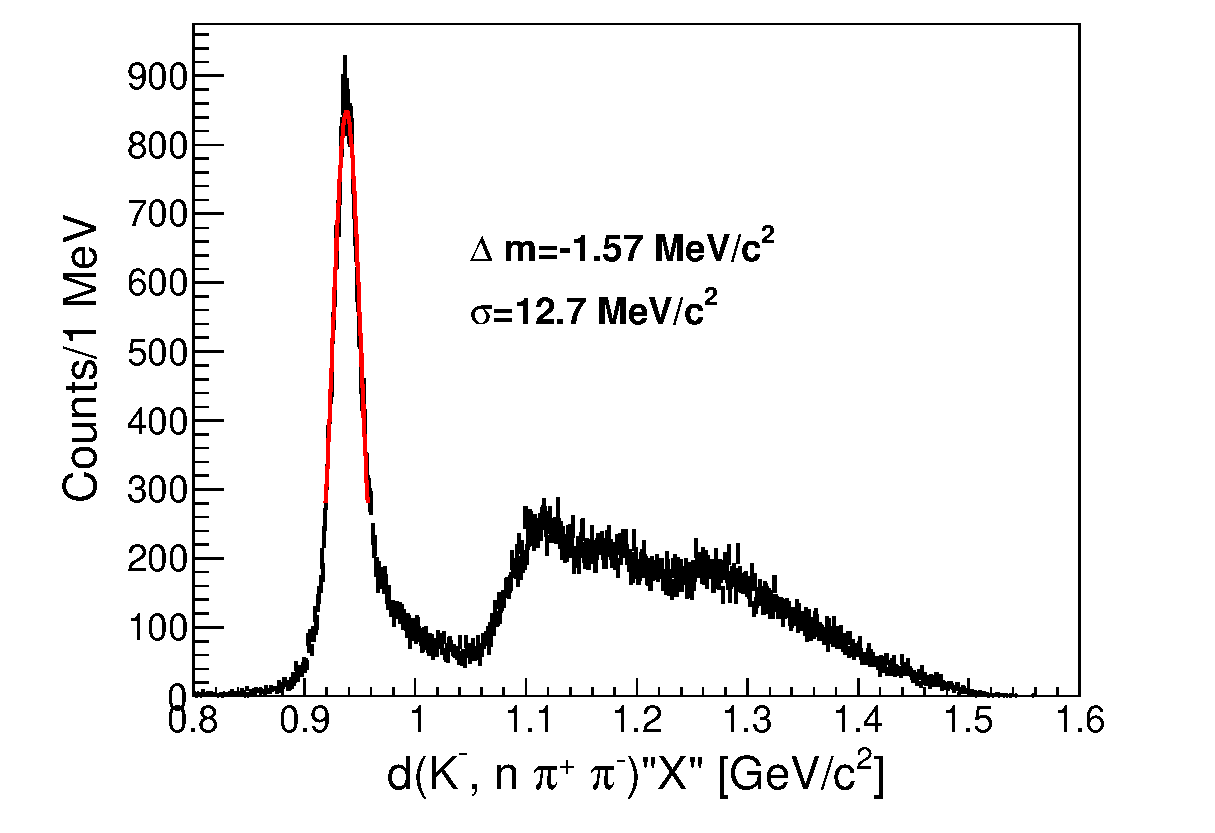
\includegraphics[width=3.5cm]{../pic/Run78/KN_ana_NC170_2sigma/KNpipi_MM_woFit.eps}
        \captionsetup{font=scriptsize}
        \caption{
          \centering
          $d(K^-, n \pi^+ \pi^-)"n"$は2$\sigma$で選ぶ。
        }
      \end{figure}
      \vspace{-5mm}
    
      \scriptsize
      期待される反応\\
      \vspace{-5mm}
      \begin{enumerate}
      \item $K^- d \rightarrow K^0 "n" n_{detected}$ 下左図で特定
      \item $K^- d \rightarrow "n" \pi \Sigma_{forward}$  $\Sigma_{forward} \rightarrow \pi n_{detected}$ \\
        下中右図で特定
      \item $K^- d \rightarrow \pi "\Sigma" n_{detected}$ 上2つ以外
      \end{enumerate}
    \end{minipage}
    \begin{minipage}{0.4\hsize}
      \begin{figure}
        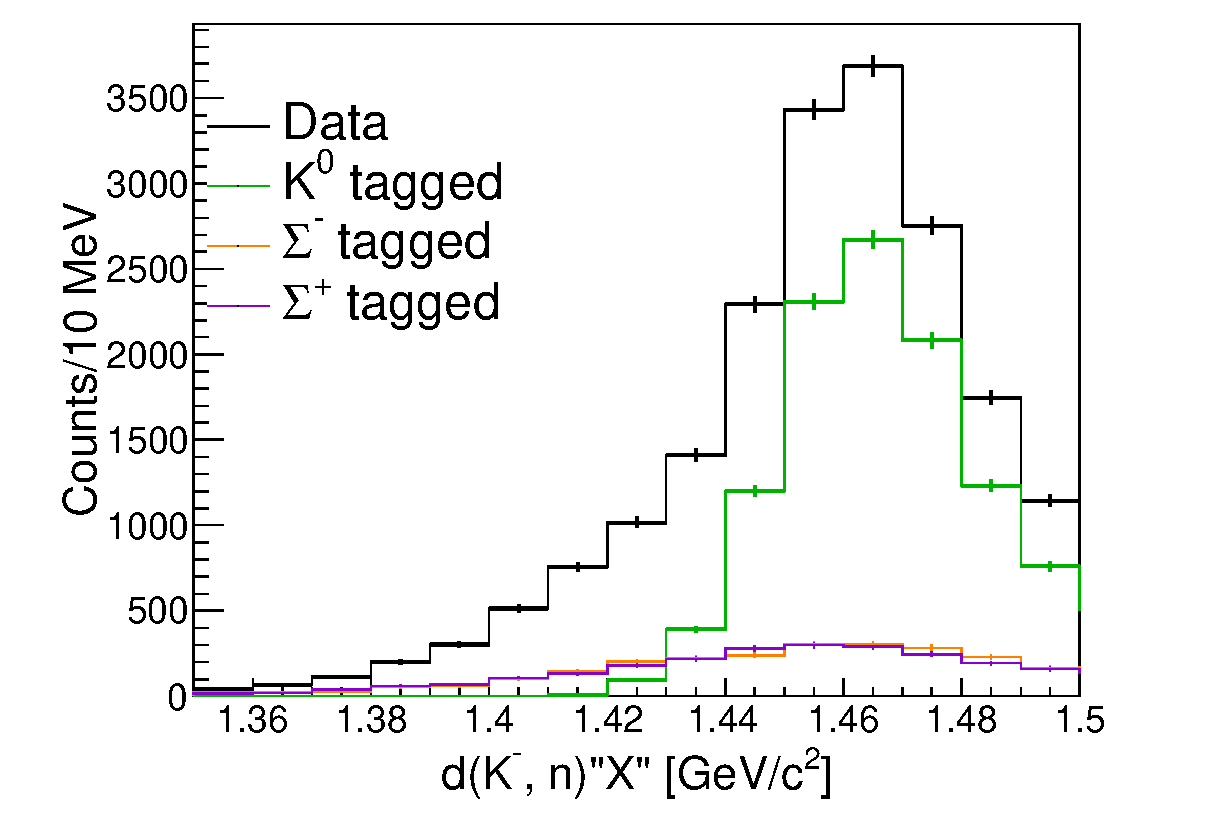
\includegraphics[width=4cm]{../pic/Run78/KN_ana_NC170_2sigma/KN_MM_all.eps}
        \captionsetup{font=scriptsize}
        \caption{
          \centering
          $d(K^-, n \pi^+ \pi^-)"n"$のイベント
        }
      \end{figure}
    \end{minipage}
  \end{tabular}

  \tminipageThree{
    \begin{figure}
      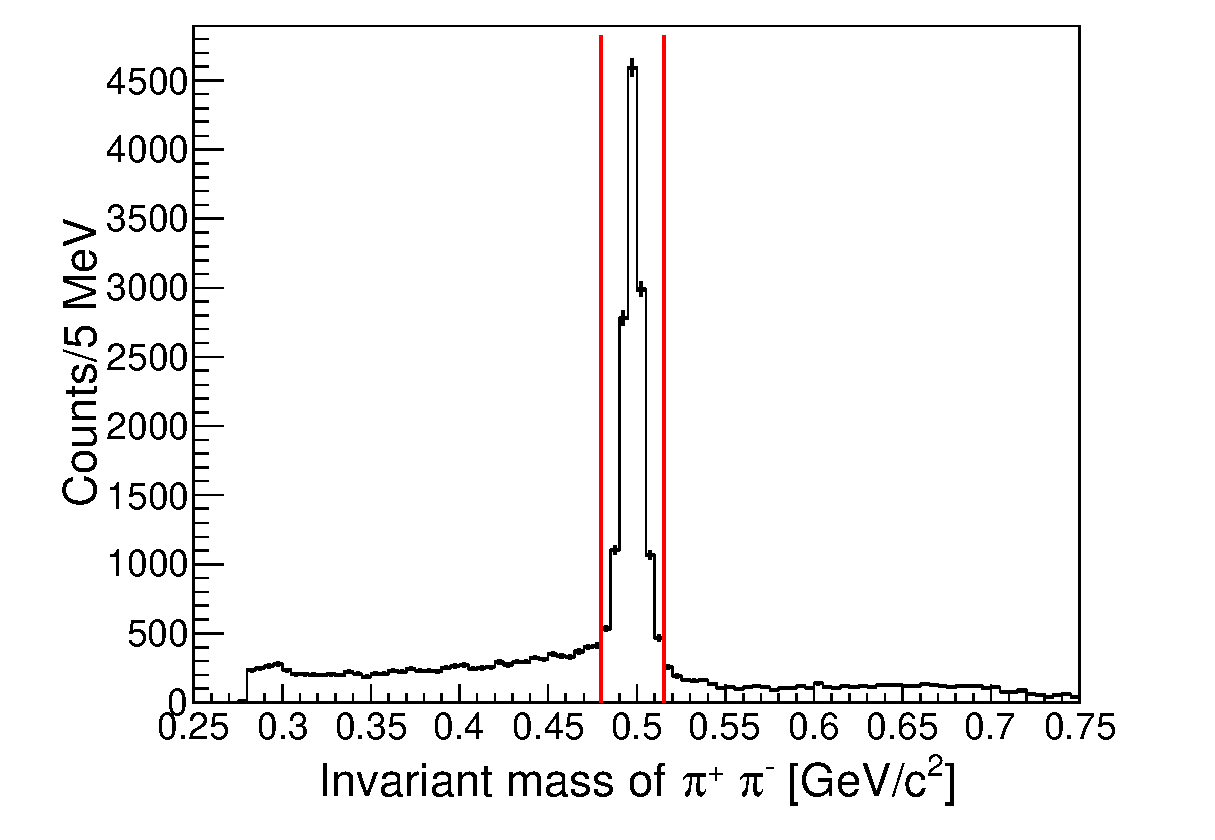
\includegraphics[width=3cm]{../pic/Run78/KN_ana_NC170_2sigma/IM_pipi_woFit.eps}
      \captionsetup{font=scriptsize}
      \caption{
        $\pi^+ \pi^-$の不変質量
      }
    \end{figure}
  }{
    \begin{figure}
      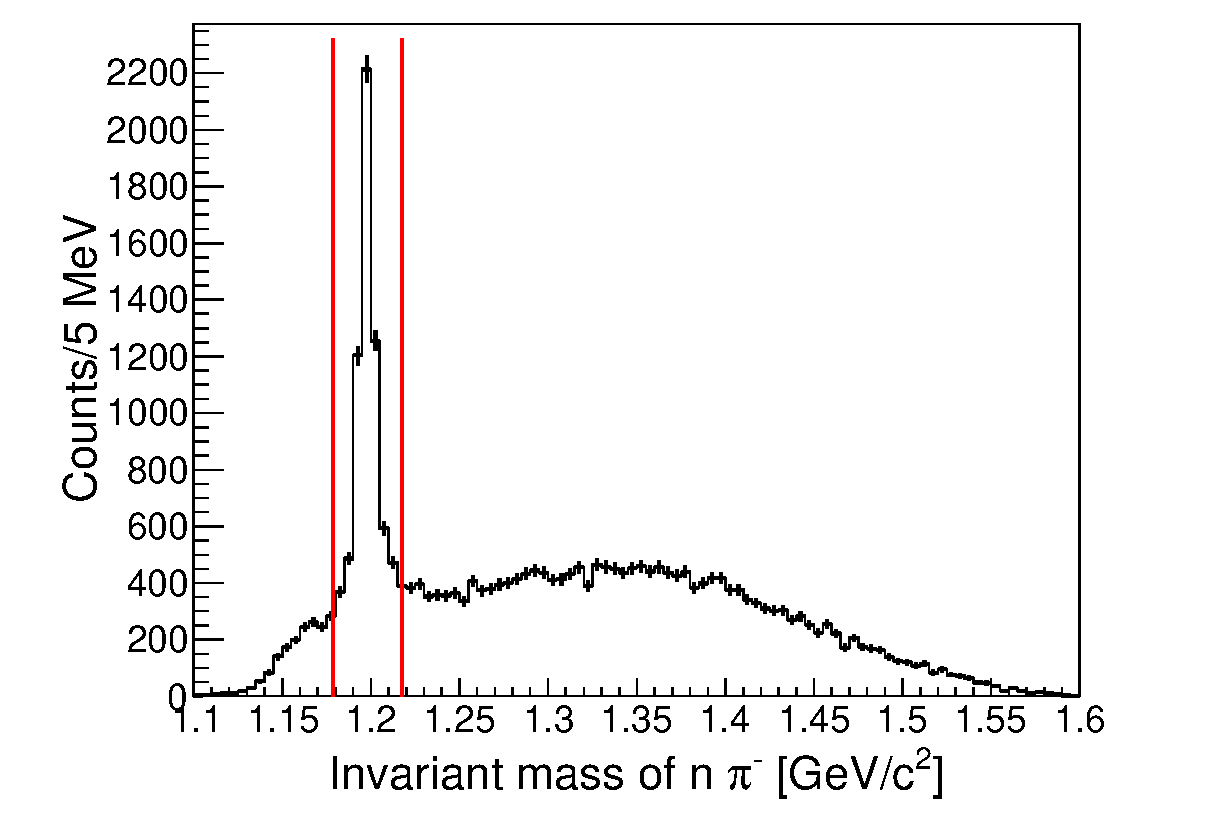
\includegraphics[width=3cm]{../pic/Run78/KN_ana_NC170_2sigma/IM_npim_woFit.eps}
      \captionsetup{font=scriptsize}
      \caption{
        $n \pi^-$の不変質量
      }
    \end{figure}
  }{
    \begin{figure}
      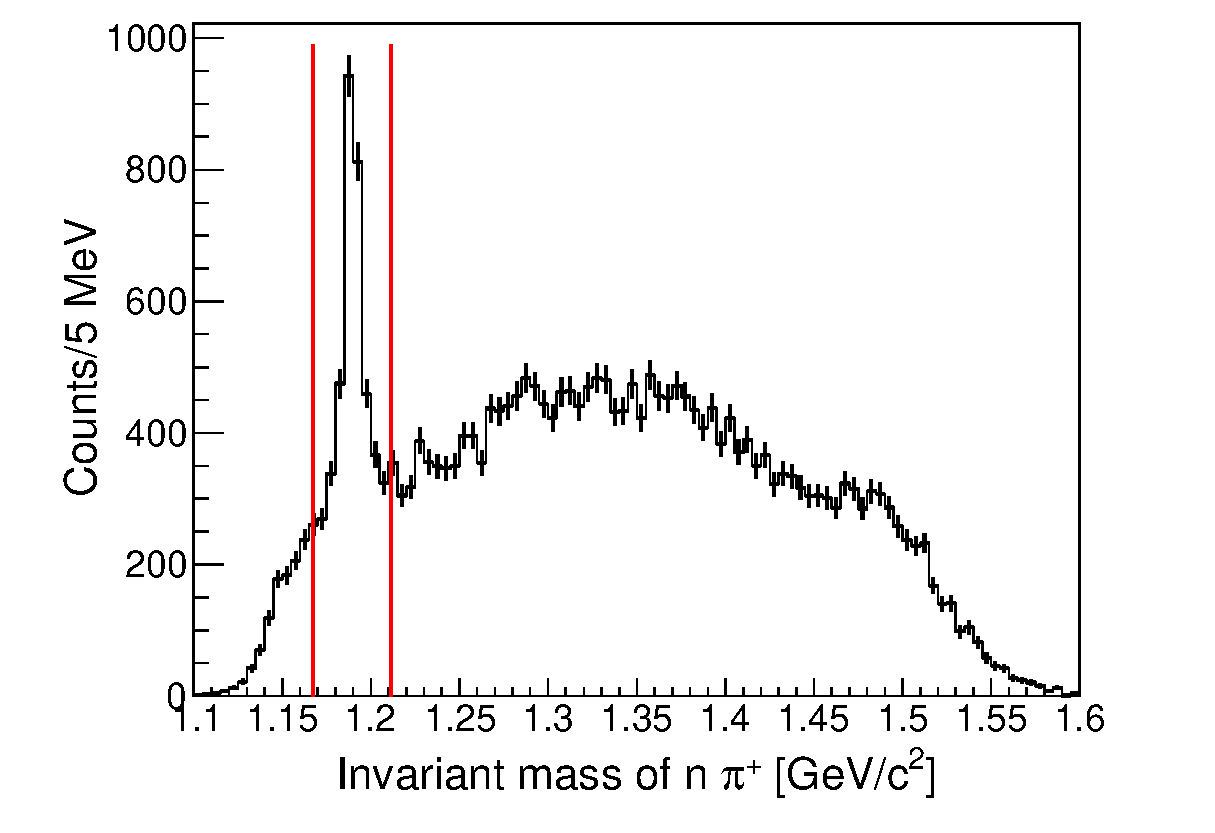
\includegraphics[width=3cm]{../pic/Run78/KN_ana_NC170_2sigma/IM_npip_woFit.eps}
      \captionsetup{font=scriptsize}
      \caption{
        $n \pi^+$の不変質量
      }

    \end{figure}
  }
  
\end{frame}
